\part{Non-singular case}

\section{$\mN=2$ $\SU(N_c)$ supersymmetric field theories}

    We consider an $\mN=2$ gauge theory with gauge group $\SU(N_c)$ and with $N_f$ hypermultiplets, i.e. $\mN=2$ SQCD with $N_c$ colors and $N_f$ flavors. Recall the following decomposition of $\mN=2$ superfields in terms of $\mN=1$ superfields:
    \begin{align}
        [\mN=2 \text{ vector multiplet}] &: V=(\lambda_\alpha,A_\mu,D)\oplus \Phi=(\phi,\psi_\alpha,F)\\
        [\mN=2 \text{ hypermultiplet}] &: Q=(H_1,\psi_{1\alpha},F_1) \oplus \tilde{Q}=(\bar{H}_2,\bar{\psi}_{2\dalpha},\bar{F}_2)
    \end{align}
    where $V$ is a vector superfield and $\Phi,H_1,H_2$ are chiral superfields. We denote by $\W_\alpha$ the chiral superfield strength associated to $V$. We have
    \begin{itemize}
        \item $V$ is a vector superfield transforming in the adjoint of $\SU(N_c)$. It belongs to $\mathfrak{su}(N_c)$ and his components are denoted by $V^a_b$ with $a,b=1,\dots,N_c$.
        \item $\Phi$ is a chiral superfield transforming in the adjoint of $\SU(N_c)$. It belongs to $\mathfrak{su}(N_c)$ and his components are denoted by $\Phi^a_b$ with $a,b=1,\dots,N_c$.
        \item $Q^i$ ($i=1,\dots,N_f$) are $N_f$ chiral superfields transforming in the $\boldsymbol{N_C}$ of $\SU(N_c)$ and in the $\boldsymbol{N_f}$ of the global group $\SU(N_f)$. It has $N_c$ components, denoted by $Q^i_a$.
        \item $\tilde{Q}_i$ are $N_f$ chiral superfields transforming in the $\bar{\boldsymbol{N_C}}$ of $\SU(N_c)$ and in the $\bar{\boldsymbol{N_f}}$ of the global group $\SU(N_f)$. It has $N_c$ components, denoted by $\tilde{Q}^a_i$.
    \end{itemize}
    $Q$ and $\tilde{Q}$ are called the \emph{quark superfields}, $H_1$ and $H_2$ the \emph{squarks} and $\phi$ the \emph{adjoint-scalar}. The lagrangian reads
    \begin{equation}
        \L^{\mN=2}_{\text{SYM}} = \frac{1}{4\pi}\Im\left[\tau\int\d^2\theta\d^2\bar{\theta}\tr\left(\Phi^\dagger e^V\Phi + Q^\dagger_i e^V Q^i + \tilde{Q}^{\dagger i}e^V \tilde{Q}_i\right)+\tau\int\d^2\theta\left(\frac{1}{2}\tr(\W^\alpha\W_\alpha)+W(\phi,H_1,H_2)\right)\right]\label{eq:lag}
    \end{equation}
    where $W(H_1,H_2)$ is the $\mN=2$ superpotential
    \begin{align}
        W(\phi,H_1,H_2) &= \sqrt{2}H_1\phi H_2 + mH_1H_2 \\
        &= \sqrt{2}(H_2)^a_i\phi^b_a (H_1)^i_b + \sqrt{2}m^i_j(H_2)^a_i(H_1)^j_a
    \end{align}
    and $\tau$ is the complexified gauge coupling
    \begin{equation}
        \tau=\frac{\theta}{\pi}+i\frac{8\pi}{g^2}.
    \end{equation}
    The matrix $m$ has to satisfy
    \begin{equation}
        [m,m^\dagger]=0
    \end{equation}
    in order to preserve $\mN=2$ supersymmetry, it is called the \emph{quark mass matrix}. This matrix can be diagonalized by an $\SU(N_f)$ transformation, i.e. a flavor rotation, to become
    \begin{equation}
        m=\text{diag}(m_1,\dots,m_{N_f}).
    \end{equation}

    Classically and with $m=0$ the global symmetry should be $\SU(N_f)\times\U(1)_B\times\U(2)_R$. The mass terms and instanton corrections breaks $\U(1)_R$ of the $R$-symmetry, leaving the compact component $\SU(2)_R$ unbroken. The lagrangian should be invariant under the latter, it is a necessary and sufficient condition to have $\mN=2$ supersymmetry. Under the unbroken $\SU(2)_R$, the bosonic fields of the vector multiplet, i.e. $A_\mu,\phi,D,F$ are singlets butthe fermions form a doublet $(\lambda_\alpha,\psi_\alpha)$. Similarly, for the hypermultiplets, the fermions $\psi_{1\alpha},\bar{\psi}_{2\dalpha}$ are singlets while their scalar superpartners for a doublet $(H_1,\bar{H_2})$. The $\SU(2)_R$ symmetry cannot be made manifest in terms of $\mN=1$ sueprfields but the symmetry $\U(1)_J\subset\SU(2)_R$ is manifest in \eqref{eq:lag}.
    
    The selection rules resulting from the breaking of the classical symmetries by mass terms and instanton corrections can be describe bt assigning symmetry transformation properties to the corresponding parameters in the action. In particular, the quark mass matrix $m$ can be decomposed into a trace part $m_S$ that transforms as a singlet under $\SU(N_f)$ and a traceless part $m_A$ that transforms in the adjoint of $\SU(N_f)$. We summarize all the representations in which the fields and the parameters transform transform in table \ref{table:fieldrepr}.

    \begin{table}[H]
        \centering
        $
        \begin{array}{c|ccccc}
            & \SU(N_c) & \SU(N_f) & \U(1)_B & \U(1)_R & \U(1)_J \\ \hline
            \Phi & \textbf{adj} & \boldsymbol{1} & 0 & 2 & 0 \\
            Q & \boldsymbol{N_c} & \boldsymbol{N_f} & 1 & 0 & 1 \\
            \tilde{Q} & \bar{\boldsymbol{N_c}} & \bar{\boldsymbol{N_f}} & -1 & 0 & 1 \\
            m_A & \boldsymbol{1} & \textbf{adj} & 0 & 2 & 0 \\
            m_S & \boldsymbol{1} & \boldsymbol{1} & 0 & 2 & 0 \\
            \Lambda^{2N_c-N_f} & \boldsymbol{1} & \boldsymbol{1} & 0 & 2(2N_c-N_f) & 0
        \end{array}
        $
        \caption{Field representations.}
        \label{table:fieldrepr}
    \end{table}

    For $\mN=2$ theories, the $\beta$ function is exact at $1$-loop and $\beta_{1\text{-loop}}\propto 2N_c-N_f$. If if $N_f<2N_c$, the $\beta$-function is negative. The theory is asymptotically free and it generates a strong-coupling scale $\Lambda$. The instanton factor is proportional to $\Lambda^{2N_c-N_f}$ and the $\U(1)_R$ symmetry is anomalous. It is broken down to a discrete $\Z_{2N_f-N_c}$ symmetry. For $N_f=2N_c$, the theory is scale invariant and $\U(1)_R$ symmetry is not anomalous. No strong-coupling scale is generated and the theory is described in terms of its bare couplings.

    $D,F,F_1$ and $F_2$ are auxiliary fields and their equations of motion are:
    \begin{align}
        F^a_b &= \pdv{W}{\phi^b_a} = \sqrt{2}(H_2)^a_i (H_1)^i_b\\
        (F_1)^a_i &= \pdv{W}{(H_{1})^i_a} = \sqrt{2}(H_2)^b_i\phi^a_b + \sqrt{2}m^j_i(H_2)^a_j,\\
        (F_2)^i_a &= \pdv{W}{(H_{2})^a_i} = \sqrt{2}\phi^b_a (H_1)^i_b + \sqrt{2}m^i_j(H_1)^j_a,\\
        D^A &= -[\phi,\phi^\dagger]^A + \bar{H}_1T^AH_1-\bar{H}_2T^AH_2
    \end{align}
    where $T^A$ are the generators of $\SU(N_f)$ and $A=1,\dots,N^2_f-1$. Note that we can also integrate out the auxiliary fields $F_1$ and $F_2$ to recast the scalar potential for the hypermultiplets as a D-term contribution. The potential reads
    \begin{align}
        V(\phi,H_1,H_2) &= \frac{1}{2}\tr(D^AD_A)+\bar{F}F+\bar{F_1}F_1+\bar{F_2}F_2\\
        &= \frac{1}{2}\tr([\phi,\phi^\dagger]^2)+\frac{1}{2}\abs{\bar{H}_1T^AH_1-\bar{H}_2T^AH_2}^2\\
        &\qquad+2\abs{(H_2)^b_i\phi^a_b+m^j_i(H_2)^a_j}^2+2\abs{\phi^b_a (H_1)^i_b+m^i_j(H_1)^j_a}^2
    \end{align}

\section{Classical moduli space}

    The D-term and F-term equations are
    \begin{figure}[H]
        \centering
        $
        \begin{array}{|cc|}
            \hline
            & \\
            D:& \begin{cases}
                \hspace{3.1cm}[\phi,\phi^\dagger]  &= 0 \\
                (H_1)^i_a(H^\dagger_1)^b_i-(H^\dagger_2)^i_a(H_2)^b_i &= \nu\delta^a_b
            \end{cases}\\
        & \\
        F:&
        \begin{cases}
            \hspace{1.3cm}(H_1)^i_a(H_2)^b_i &= \rho\delta^b_a \\
            (H_1)^j_am^i_j+\phi^b_a(H_1)^i_b &= 0 \\
            m^i_j(H_2)^a_j+(H_2)^b_i\phi^a_b &= 0
        \end{cases}\\
        & \\ \hline
        \end{array}
        $
    \end{figure}
    \todo{Verify how to obtain these equation from the F-terms and D-terms}
    where $\nu$ and $\rho$ are arbitrary complex numbers.\todo{From where do those come from ?} The the two equations in the D-terms appear separately is a consequence of $\mN=2$ supersymmetry. One can square the D-term and show that the cross-term cancels or by noting that the first term is an $\SU(2)_R$-singlet and that that the second is part of a triplet\footnote{More generally, we will need to quotient by the complexified gauge transformation, which can be used to diagonalize $\phi$ and the first equation is automatically satisfied. This is another explanation.}.
    
    These equations suggest that $\phi,H_1$ and $H_2$ may get VEVs, which we denote by $\vev{\phi},\vev{H_1}$ and $\vev{H_2}$ respectively. Since there $N^2_c-1$ components $\phi^a_b$, $N_c\cdot N_f$ components $(H_1)^i_a$ and $N_c\cdot N_f$ components $(H_2)^a_i$, there are $N_c(N_c+2N_f)-1$ complex scalars in total. Meaning that the D-term and F-term equations define a subspace of $\C^{N_c(N_c+2N_f)-1}$. The \emph{classical moduli space} is defined as
    \begin{equation}
        \M_c\equiv Z(F,D)/G\subset \C^{N_c(N_c+2N_f)-1}
    \end{equation}
    where $G=\SU(N_c)$ is the gauge group. It turns out that we can just consider the F-term equations if we quotient by the complexified gauge group:
    \begin{equation}
        \M_c = Z(F)/G_\C.
    \end{equation}

    The solutions to those equations fall into various branches corresponding to the phases of the theory. The \emph{Coulomb branch} is the region of the moduli space where only the scalars from the vector multiplet can take VEVs, i.e. where $\vev{H_1}=\vev{H_2}=0$. The \emph{Higgs branch} is the region of the moduli space where only the scalars from the hypermultiplets can take VEVs, i.e. where $\vev{\phi}=0$. \emph{Mixed branches} are regions where all VEVs are non-vanishing. For simplicity we will mostly consider the case with no mass: $m^i_j=0$.

    \subsection{Coulomb branch}

        The only non-trivial equation is the first D-term equation $[\phi,\phi^\dagger]=0$, the other four are automatically satisfied. This equation is if and only $\phi$ belongs to $\mathfrak{h}_\C$, the complexified Cartan subalgebra of $\mathfrak{su}(N_c)$. In our case, this means that the scalar fields matrix $\phi$ can be diagonalized using a color rotation and put in the form
        \begin{equation}
            \phi = \sum_I \phi_Ih^I
        \end{equation}
        where $h^I=E_{I,I}-E_{I+1,I+1}$ with $(E_{I,J})_{ab}=\delta_{aI}\delta{bJ}\equiv$ are the generators of the Cartan subalgebra and $I=1,\dots N_c-1$ ($N_c-1$ is the rank of $\mathfrak{su}(N_c)$). In simpler words, the vacuum configurations are of the form
        \begin{equation}
            \phi=\text{diag}(\phi_1,\dots,\phi_{N_c}),\qquad \sum^{N_c}_{a=1}\phi_a=0.\label{eq:diagform}
        \end{equation}
        The vacuum configurations then depend on $N_c-1$ complex numbers so the Coulomb branch is a quotient of $\C^{N_c-1}$.
        
        At a generic point, the gauge group is broken to $\U(1)^r\times W$, where $W_G$ is the Weyl group of the gauge group, the group of residual gauge symmetries, while acting on $\phi$, do not not take it out of the Cartan subalgebra, i.e. keeps it the form \eqref{eq:diagform}. The low energy dynamic is the that of $r$ massless vector multiplets and $\dim G-r$ massive ones, with masses depending on the specific VEV's. The Weyl group of $\SU(N_c)$ is $S_{N_c-1}$. At last, the classical Coulomb branch is
        \begin{equation}
            \boxed{\M^V_c=\frac{\C^{N_c-1}}{S_{N_c-1}}.}
        \end{equation}
        A natural set of $\U(1)^{N-1}\times S_{N-1}$ invariant coordinates on this $(N_c-1)$-dimensional Coulomb branch can be shown to be
        \begin{equation}
            u_2=\sum_{i<j}\phi_i\phi_j,\quad u_3=\sum_{i<j<k}\phi_i\phi_j\phi_k,\quad \dots,\quad u_{N_c}=\phi_1\dots \phi_{N_c}, \qquad i,j,k=1,\dots,N_c.
        \end{equation}
        It has an orbifold singularity along submanifolds where some of the $\phi_a$'s are equal. In this case, some of the non-abelian gauge symmetry is restored. The scalar potential gives the mass of the fields $H_1$ and $H_2$ as $\phi_a+m_i$. The vanishing of these masses describes a complex co-dimension $1$ submanifold of the Coulomb branch. 

    \subsection{Higgs branch}

        Since we consider a vanishing quark mass matrix, only the second D-term equation and the first F-term equation are non-trivial. Recall that the squark fields $H_1$ and $H_2$ are complex matrices of size $N_c\times N_f$ and $N_f\times N_c$ respectively:
        \begin{equation}
            H_1=
            \begin{bmatrix}
                (H_1)^1_1 & \dots & (H_1)^{N_f} \\
                \vdots & & \vdots \\
                (H_1)^1_{N_c} & \dots & (H_1)^{N_f}_{N_c}
            \end{bmatrix},\qquad
            (H_2)^t=
            \begin{bmatrix}
                (H_2)^1_1 & \dots & (H_2)^{N_f} \\
                \vdots & & \vdots \\
                (H_2)^1_{N_c} & \dots & (H_2)^{N_f}_{N_c}
            \end{bmatrix}.
        \end{equation}

        \subsubsection{Squark VEV solutions}

            \begin{itemize}
                \item \underline{$N_f\geq2N_c$:} any solution can be put using flavor and color rotations:
                \begin{align}
                    \begin{split}
                    H_1 &= 
                    \begin{bmatrix}
                        \kappa_1 & & & 0 & & & 0 & \\
                        & \ddots & & & \ddots & & & \ddots \\
                        & & \kappa_{N_c} & & & 0 & & 
                    \end{bmatrix},\\
                    (H_2)^t &= 
                    \begin{bmatrix}
                        \tilde{\kappa}_1 & & & \lambda_1 & & & 0 & \\
                        & \ddots & & & \ddots & & & \ddots \\
                        & & \tilde{\kappa}_{N_c} & & & \lambda_{N_c} & & 
                    \end{bmatrix}
                \end{split}\label{eq:Higgsbranchsol}
                \end{align}
                where
                \begin{align}
                    \kappa_a\tilde{\kappa}_a &= \rho,\qquad\rho\in\C \label{eq:Higgsbrachcdt1}\\
                    \lambda^2_a &= \kappa^2_a-\frac{\abs{\rho}^2}{\kappa^2_a}+\nu,\qquad\nu\in\R \label{eq:Higgsbrachcdt2}
                \end{align}
                and the $\kappa_a's$ are non-zero if $\rho$ is non-zero.
                \item \underline{$N_f<2N_c$:} starting from a solution for $N_f=2N_c$ with some vanishing flavor columns, one can always construct a solution for $N_f<2N_c$ by removing those columns. On the other hand, starting from a solution for $N_f<2N_c$, one can always add vanishing flavor columns th construct a solution for $N_f=2N_c$. The necessary flavor rotation to put the solution into the form \eqref{eq:Higgsbranchsol} can be chosen not to act on these extra columns of zeros. This ensures us that this column-reduction procedure from $N_f=2N_c$ solutions will generate an $N_f<2N_c$ solution in every flavor orbit.
                
                To reduce \eqref{eq:Higgsbranchsol} by $2N_c-N_f$ columns, we must set $2N_c-N_f$ parameters to zero: $\lambda_1=\dots=\lambda_i=\kappa_1=\dots=\kappa_j=0$ with $i+j=2N_c-N_f$. By \eqref{eq:Higgsbrachcdt1}-\eqref{eq:Higgsbrachcdt2}, if some $\kappa$'s vanish, we must set $\rho=0$ before, which implies that some $\lambda_a$'s vanish too. Consequently, there are two possibilities to reducing columns, hence defining two sub-branches of the Higgs branch:
                \begin{itemize}[label=$\triangleright$]
                    \item \emph{baryonic branch}: only some $\lambda_a$'s vanish, more precisely, $i=2N_c-N_f$ and $j=0$. Starting from the case $N_f=2N_c$ and  the last $2N_c-N_f$ $\lambda_a$'s to zero: $\lambda_{N_f-N_c+1}=\dots=\lambda_{N_c}=0$. The $\kappa_a$'s and the $\lambda_a$'s are related by \eqref{eq:Higgsbrachcdt2}, which implies that the last $2N_c-N_f$ $\kappa_a$'s are completely fixed in terms of $\rho$ and $\nu$. Let us call this value $\kappa_0$. The same goes for the $\tilde{\kappa}_a$'s and we have
                    \begin{align}
                        \begin{split}
                        H_1 &= 
                        \begin{bmatrix}
                            \kappa_1 & & & & & & \phantom{\lambda_1} & & \\
                            & \ddots & & & & & & \phantom{\ddots} & \\
                            & & \kappa_{N_f-N_c} & & & & & & \phantom{\lambda_{N_f-N_c}} \\
                            & & & \kappa_0 & & & & & \\
                            & & & & \ddots & & & & \\
                            & & & & & \kappa_0 & & &
                        \end{bmatrix},\qquad\kappa_a\in\R^+\\
                        (H_2)^t &= 
                        \begin{bmatrix}
                            \tilde{\kappa}_1 & & & & & & \lambda_1 & & \\
                            & \ddots & & & & & & \ddots & \\
                            & & \tilde{\kappa}_{N_f-N_c} & & & & & & \lambda_{N_f-N_c} \\
                            & & & \tilde{\kappa}_0 & & & & & \\
                            & & & & \ddots & & & & \\
                            & & & & & \tilde{\kappa}_0 & & &
                        \end{bmatrix},\qquad\lambda_a\in\R^+\\
                    \end{split}\label{eq:barynoicbranch}
                    \end{align}
                    where
                    \begin{align}
                        \kappa_a\tilde{\kappa}_a &= \rho,\qquad\rho\in\C\\
                        \lambda^2_a &= \kappa^2_a-\kappa^2_0+\abs{\rho}^2\left(\frac{1}{\kappa^2_a}-\frac{1}{\kappa^2_0}\right),\qquad\nu\in\R 
                    \end{align}
                    Since there are only $N_c$ $\lambda_a$'s in the first place, there are only $N_c$ of them to set $0$ so this method only works if $N_f\geq N_c$. For reasons that will become clear later, we use the term baryonic branch for the $N_f\geq 2N_c$ solutions \eqref{eq:Higgsbranchsol} as well.
                    
                    One can see that the opposite case, i.e. taking only $\kappa_a$'s to vanish, with $i=0$ and $j=2N_c-N_f$, leads to a submanifold of the same branch upon interchanging $H_1$ and $H_2$, which is a symmetry (charge conjugation) of our theory, as one can also see from the F-term and D-term equation for example.

                    \item \emph{non-baryonic branch}: we now set both some $\lambda_a$'s and some $\kappa_a$'s to zero, more precisely we set $\lambda_1=\dots=\lambda_i=\kappa_1=\dots=\kappa_j=0$ with $i,j\neq0$ and $i+j=2N_c-N_f$. From the constraints \eqref{eq:Higgsbrachcdt1}-\eqref{eq:Higgsbrachcdt2}, this implies that $\rho=\nu=0$ and $\kappa_a=\lambda_a$. The VEVs have the form
                    \begin{align}
                        \begin{split}
                            H_1 &= 
                            \begin{bmatrix}
                                \kappa_1 & & & 0 & & & 0 & \\
                                & \ddots & & & \ddots & & & \ddots \\
                                & & \kappa_r & & & 0 & & \\
                                & & & & & & & \\
                                & & & & & & &
                            \end{bmatrix},\\
                            (H_2)^t &= 
                            \begin{bmatrix}
                                0 & & & \kappa_1 & & & 0 & \\
                                & \ddots & & & \ddots & & & \ddots \\
                                & & 0 & & & \kappa_r & & \\
                                & & & & & & & \\
                                & & & & & & &
                            \end{bmatrix},\qquad\kappa_a\in\R^+\\
                        \end{split}\label{eq:nonbarynoicbranch}
                    \end{align}
                    where $r\leq \lfloor N_f/2\rfloor$ and $2N_c-N_f$ columns of zeros should be deleted by the column-reduction procedure. 
                    
                    If $N_f$ is odd, there remains at least one column of zeros in the reduced matrices. The different values of $r$ give distinct submanifolds of the branch with maximal value. Nonetheless, we will refer to them as different baryonic branches for reasons that will become clear later.
                    
                    Some non-baryonic branches can also be obtained as submanifolds of the baryonic branch by setting $\rho=\kappa_0=\tilde{\kappa}_0=0$ in \eqref{eq:barynoicbranch}. The reason for these choices of terminology will become clear latter. Non-baryonic branches exist for $N_f\geq2$, for $N_f<2$ there is no Higgs branch at all.
                \end{itemize}
            \end{itemize}
        
        \subsubsection{Gauge symmetry and separate branches}

            Let us clarify the intersection pattern of the Higgs branches. We say that two Higgs branches are \emph{separate} if any path between the two goes through a point of enhanced gauge symmetry. This implies in particular that branches that if a branch has a larger unbroken gauge group than the other, they separate.

            \underline{Baryonic branch:} the $N_f\geq2N_c$ solution \eqref{eq:Higgsbranchsol} and the $N_f\leq2N_c$ solution \eqref{eq:barynoicbranch} completely break the gauge symmetry. By the Higgs mechanism, there $N^2_c-1$ hypermultiplets that become massive so the number of massless hypermultiplets is $\H=N_fN_c-(N^2_c-1)$. This counts the quaternionic dimension of the Higgs branch. There are submanifolds of the baryonic branch where the gauge symmetry is enhanced. These occur when two or more rows of $H_1$ and $H_2$ vanish, i.e. if $\rho=\nu=0$ for \eqref{eq:Higgsbranchsol} and if $\rho=\kappa_0=0$ for \eqref{eq:barynoicbranch}, giving rise to non-baryonic branch VEV's \label{eq:nonbarynoicbranch} with
            \begin{equation}
                r\leq \min\{N_f-N_c,N_c-2\}.\label{eq:rrange}
            \end{equation}

            \underline{Non-baryonic branch:} there are non-baryonic branches with $r$ outside of the range \eqref{eq:rrange}. Recall that the gauge group acts on the columns so, at a generic point, the unbroken gauge group is $\SU(N_c-r)$. 
            
            with $N_f-2r$ massless hypermultiplets in the fundamental. There are different unbroken gauge groups for different values of $r$ so they are separate branches. The Higgs mechanism gives mass to $2N_cr-r^2$ hypermultiplets\footnote{Since $\dim\SU(N_c)-\dim\SU(N_c-r)=2N_cr-r^2$.} therefore there are $\H=r(N_f-r)$ massless multiplets neutral under the unbroken gauge group.

        \subsubsection{Flavor symmetry}

            To identify the unbroken global symmetries on the Higgs branches, it is useful to define a basis of gauge-invariant quantities made from the squark VEV's:
            \begin{align}
                M^i_j &\equiv (H_2)^a_j(H_1)^i_a\\
                B^{i_1\dots i_{N_c}} &\equiv \eps^{a_1\dots a_{N_c}}(H_1)^{i_1}_{a_1}\dots(H_1)^{i_{N_c}}_{a_{N_c}}\\
                \tilde{B}_{i_1\dots i_{N_c}} &\equiv \eps_{a_1\dots a_{N_c}}(H_2)^{a_1}_{i_1}\dots(H_2)^{a_{N_c}}_{i_{N_c}}.
            \end{align}
            $M$ is called the \emph{meson field} and $B,\tilde{B}$ are called the \emph{baryon fields}. The latter are only defined for $N_f\geq N_c$.

            \underline{The baryonic branch:} on this branch, the baryonic fields are non-vanishing: $B,\tilde{B}\neq0$, hence the name, and from \eqref{eq:Higgsbranchsol} or \eqref{eq:barynoicbranch}, the meson field is
            \begin{equation}
                M=
                \begin{bmatrix}
                    \rho & & & \kappa_1\lambda_1 & & & 0 & \\
                    & \ddots & & & \ddots & & & \ddots \\
                    & & \rho & & & \kappa_{N_c}\lambda_{N_c} & & \\
                    & & & & & & & \\
                    & & & & & & &
                \end{bmatrix}\label{eq:baryonicbranchmesonfield}
            \end{equation}
            where the $\rho$-block is $N_c\times N_c$. For $N_f\leq 2N_c$ we should remove the appropriate number of columns from the right and rows from the bottom.
            
            For $N_f\geq 2N_c$, the meson field \eqref{eq:baryonicbranchmesonfield} and the non-vanishing baryon VEV's imply that the global symmetry is broken as
            \begin{equation}
                \SU(N_f)\times\U(1)_B\times\SU(2)_R\to\U(N_f-2N_c)\times\U(1)^{N_c-1}\times\SU(2)'_R.
            \end{equation}
            The number of real Goldstone boson bosons is then $\G=4N_fN_c-N^2_c-N_c+1$. Since the number of real parameters describing the Higgs branch in \eqref{eq:Higgsbranchsol} is $\mP=N_c+3$, we can see that $\G+\mP=4\H$. This is a check that we have a complete parametrization of this branch.

            For $N_C\leq N_f< 2N_c$, the global symmetry is broken as
            \begin{equation}
                \SU(N_f)\times\U(1)_B\times\SU(2)_R\to\SU(2N_c-N_f)\times\U(1)^{N_c-N_c}\times\SU(2)'_R.
            \end{equation}
            The number of real Goldstone boson is then $\G=-4N^2_c+4N_cN_f-N_f+N_c+1$. The number of real parameters describing the baryonic branch is $\mP=N_f-N_c+3$ and $\G+\mP=4\H$.

            \underline{The non-baryonic branches:} on these branches, the baryonic field vanishes, $B=\tilde{B}=0$, hence their name, and the meson field is given by
            \begin{equation}
                M=
                \begin{bmatrix}
                    0 & & & \kappa^2_1 & & & 0 & \\
                    & \ddots & & & \ddots & & & \ddots \\
                    & & 0 & & & \kappa^2_r & & \\
                    & & & & & & & \\
                    & & & & & & &
                \end{bmatrix}\label{eq:nonbaryonicbranchmesonfield}
            \end{equation}
            where the first block of zeros is $r\times r$. This implies that the global symmetry is broken as
            \begin{equation}
                \SU(N_f)\times\U(1)_B\times\SU(2)_R\to\U(N_f-2r)\times\U(1)^{r}\times\SU(2)'_R.
            \end{equation}
            The number of real Goldstone bosons is $\G=r(4N_f-4r-1)$ and $\mP=r$ so $\G+\mP=4\H$.

        \subsubsection{Gauge-invariant description}

            The configuration \eqref{eq:Higgsbranchsol} is sent to inequivalent points in the moduli space, but with the same physics, by global symmetry transformations. Gauge symmetry transformations on the other hand, sends them to equivalent point in the moduli space, which is not manifest in our writing. We want to describe the moduli space in terms of gauge-invariant coordinates, i.e. describe the various branches in terms of constraints on the meson field and the baryonic fields.

            The Higgs branch is a hyperKähler quotient of the squark space by the gauge group, with the D-terms and F-terms as moment maps. It is easier to work with a Kähler quotient, thus consider the theory as an $\mN=1$ theory with a superpotential interaction. In a Kähler quotient, the D-term equations are equivalent to quotienting by the complexified gauge group. This can be achieved by expressing the VEVs directly in terms of holomorphic gauge-invariant coordinates, such as the meson and baryonic fields, and by imposing the F-term equations. The non-trivial structure of the quotient is manifest in the fact that the gauge invariant coordinates are not independent as functions of the squark fields but they satisfy a set of polynomial relations which we must impose as constraints. Our goal is to find a set of generators of for these constraints and the F-term equations.

            By definition, the meson field $M$ and the baryonic fields $B,\tilde{B}$ must satisfy
            \begin{equation}
                B^{i_1\dots i_{N_c}}\tilde{B}_{j_1\dots j_{N_c}}=M^{[i_1}_{j_1}\dots M^{i_{N_c}]}_{j_{N_c}}
            \end{equation}
            which can be rewritten as
            \begin{equation}
                (\star B)\tilde{B}=\star(M^{N_c})\label{eq:constraint1}
            \end{equation}
            with $(\star B)_{i_{N_c+1}\dots i_{N_f}}=\eps_{i_1\dots i_{N_f}}B^{i_1\dots i_{N_c}}$.
            
            Also, since any expression antisymmetrized on $N_c+1$ color indices must vanish, any product of $M$'s, $B$'s and $\tilde{B}$'s antisymmetrized on $N_c+1$ upper or lower indices must vanish. For $B,\tilde{B}\neq0$, an induction argument shows that the constraint \eqref{eq:constraint1} together with
            \begin{equation}
                M\cdot\star B=M\cdot\star\tilde{B}=0\label{eq:constraint2}
            \end{equation}
            where $\cdot$ represents the contraction of flavor indices. If $B=\tilde{B}=0$, all the other constraints are automatically satisfied and \eqref{eq:constraint1} implies \eqref{eq:constraint2}

            From \eqref{eq:constraint1} and \eqref{eq:constraint2}, one can show that
            \begin{equation}
                \text{rank}(M)\leq N_c.
            \end{equation}

            The first F-terms gives two new constraints:
            \begin{align}
                M'\cdot B = \tilde{B}\cdot M' &= 0\label{eq:constraint3}\\
                M\cdot M' &= 0\label{eq:constraint4}
            \end{align} 
            and the other two equations are relevant only for mixed branches. Finally, a complete set of constraints is given by \eqref{eq:constraint1},\eqref{eq:constraint2},\eqref{eq:constraint3} and \eqref{eq:constraint4}.

            The condition \eqref{eq:constraint4} is already quite restrictive; its only solutions are, up to flavor rotations, the meson field configuration \eqref{eq:baryonicbranchmesonfield} and \eqref{eq:nonbaryonicbranchmesonfield}. NThe non-baryonic solutions have rank $r\leq\lfloor N_f/2\rfloor$. For $N_f> 2N_c$, this will be reduced to $r\leq N_c$ by \eqref{eq:constraint2}. For $N_f\leq 2N_c$ on the other hand this constraint is automatically satisfied and \eqref{eq:constraint2} is implied by \eqref{eq:constraint4}.

    \subsection{Mixed branches}

        Up until now, we have not taken the last two F-term equation into account. Whether or not the masses vanish, it has no effect on the Coulomb branch. For the Higgs branch on the other hand, it has no effect on it if and on ly the masses vanish, otherwise they put constraints on the Higgs VEVs and lifts the branch. Indeed, there are non non-zero masses for which the generic Higgs branch \eqref{eq:Higgsbranchsol} for $N_f=2N_c$ satisfies the last two F-term equations. Since the Higgs phase corresponds to flat directions along which some components of the hypermultiplet remain massless, we say that the presence of mass terms ``lifts'' these flat directions.

        For mixed branches, i.e. when all both $H_1$ or $H_2$ and $\phi$ take non-vanishing VEVs, those equations are always important, even if the masses are vanishing. We suppose again that it is the case. Once again, $\phi$ can be diagonalized using color rotations. Then the last two F-term equations only have non-zero solution for $H_1,H_2$ and $\phi$ if the squarks and adjoint-scalar VEVs live in disjoint color subgroups. This leads to a clean distinction between the Higgs branches: branches with different gauge groups are distinct between because they appear as the Higgs factor of mixed branches with manifestly distinct Coulomb factors.

        The other F-term and D-terms equations then implies that the VEVs can be parametrized up to gauge and flavor rotations as
        \begin{equation}
            \Phi=\text{diag}(0,\dots,0,\phi_{r+1},\dots,\phi_{N_c}),\qquad \phi\in\C,\qquad\sum_a\phi=0
        \end{equation}
        and as in \eqref{eq:nonbarynoicbranch} for the squarks. We conclude that locally, the mixed branch has the structure of a direct product of a non-baryonic Higgs branch and a Coulomb branch. This Coulomb branch can be identified with the Coulomb branch of the unbroken $\SU(N_c-r)$ gauge theory of the non-baryonic Higgs branch. Henceforth, we will refer to the mixed branch as a non-baryonic branch.

    \subsection{Summary}

        We summarize by recording the number $\V$ of massless $\U(1)$ vector multiplets and $\H$ of massless neutral hypermultiplets at a generic point of the moduli space:
        \begin{figure}[H]
            \centering
            $
            \begin{array}{c|c|c|c}
                & \text{exists when} & \V & \H \\ \hline
                \text{Barynoic branch} & N_f\geq N_c & 0 & N_fN_c-N^2_c+1 \\
                \text{Non-baryonic branch} & N_f\geq 2 & N_c-1-r & r(N_f-r) \\
                \text{Coulomb branch} & / & N_c-1 & 0
            \end{array}
            $
        \end{figure}
        where $1\leq r\leq \min\{\lfloor N_f/2\rfloor,N_c-2\}$. The Higgs branch intersect the Coulomb branch at the origin and, out of the Higgs branch, emanates various mixed branch which touch the Coulomb branch along submanifolds where two or more squarks are massless, which where a non-abelian gauge group is unbroken. 
        \begin{itemize}
            \item \textbf{Non-baryonic--Coulomb:} the non-baryonic branch intersects the Coulomb branch along a submanifold $B$. On $B$, classically, there is an $\SU(r)\times\U(1)^{N_c-r}$ unbroken gauge group with $N_f$ massless hypermultiplets in the fundamental representation of $\SU(r)$ and charged under the one of the $\U(1)$ factors (by an appropriate choice of basis of the $\U(1)'s$). 
            \item \textbf{Baryonic--Coulomb:} the baryonic branches intersect the Coulomb branch at its origin. There, classically, the full $\SU(N_c)$ is unbroken with $N_f$ massless fundamental flavors.
            \item \textbf{Non-baryonic--Baryonic:} the various Higgs branches connect up along a submanifold of enhanced gauge symmetry. In particular, the baryonic intersects the non-baryonic branch along a submanifold $A$ with enhanced gauge group $\SU(N_c-r)$ for $r\leq \min\{\lfloor N_f/2\rfloor,N_c-2\}$.
        \end{itemize}
        
        \begin{figure}[H]
            \centering
            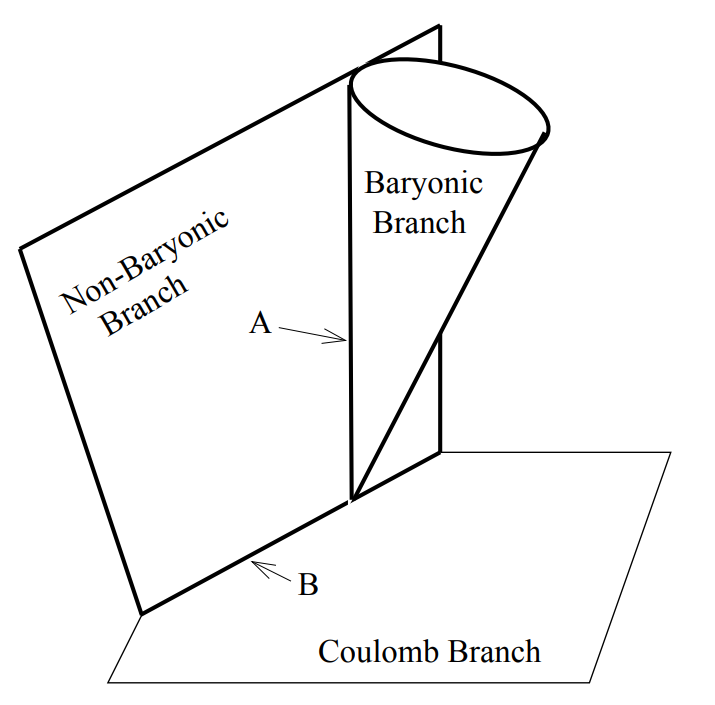
\includegraphics[scale=0.3]{Pictures/classicalmodulispace.png}
            \caption{Map of the classical moduli space of $\mN=2$ $\SU(N_c)$ SQCD with $N_f$ fundamental flavors, from \cite{Argyres_1996}.}
        \end{figure}

\section{Quantum moduli space}

\section{Quantum Higgs branches and the non-renormalization theorem}

\section{Higgs branch roots}

    \subsection{Non-baryonic root}

    \subsection{Baryonic root}

\part{$A_1$ singularity}

\part{$A_n$ singularity}

\part{$\D_4$ singularity}